\chapter{Resultados}
\label{resultados}

\section{GFED}

\subsection{\textit{Random Forest}}

\textit{Random Forest} é um dos modelos de algoritmo mencionado no capítulo 3. Modelos
\textit{Random Forest} são escolhidos para produzir boas previsões que são fáceis de entender. O fato de que pode lidar com grandes conjuntos de dados com eficiência e fornecer um alto nível de precisão geral é uma das razões pelas quais o escolhemos para verificar a eficácia de técnicas de aprendizado de máquina dentro do nosso problema.

\subsection{\textit{Multi-Layer Perceptron}}

MLP é um modelo de perceptron mencionado no capítulo 3. Esta arquitetura é muito
configurável, principalmente quando construída a partir de um \textit{framework} como o Pytorch. No entanto, esta maleabilidade também proporciona muitos pontos de falha, como bugs ou dificuldades de implementação.

Redes como o MLP tendem a lidar melhor com dados contínuos e a terem dificuldades
em interpretar dados categóricos, o que traz outros desafios na adaptação do conjunto de
dados para esta arquitetura.

\subsection{Metodologia}

Podemos descrever o funcionamento do códigos de treinamento dos modelos por meio do seguinte fluxograma, na figura \ref{fig:rfflux}:

\begin{figure}[H]
	\centering
	\begin{minipage}{0.98\linewidth}
		\centering
		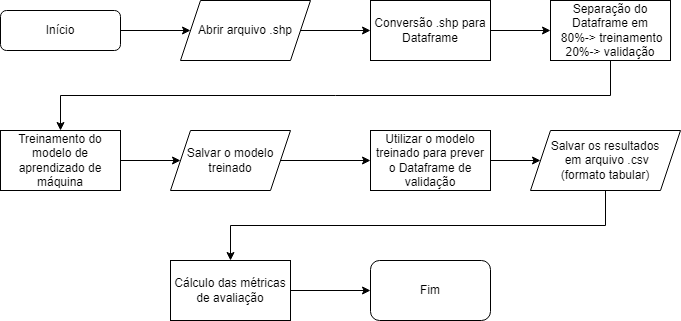
\includegraphics[width=\linewidth]{tg1/figuras/fluxograma_gfed.png}
		\caption{Fluxograma do funcionamento dos códigos de treinamento} \label{fig:rfflux}
	\end{minipage}
\end{figure}

Os parâmetros utilizados para a função do \textit{Random Forest Classifier} foram os valores padrões utilizados pelo scikit-learn \cite{sklearnrfc}, com o objetivo de obter-se um primeiro resultado para o nosso modelo. Enquanto os parâmetros do MLP foram sendo definidos até que a rede apresentasse \textit{overfitting}, demonstrando capacidade de generalização. Após isto, os seus hiper-parâmetros foram ajustados até fossem atingidos os melhores resultados encontrados.

\subsection{Desempenho}

Na última etapa de calculo da precisão do modelo Random Forest, foi obtido os
valores da tabela \ref{tab:rf} para quando classificamos o dataframe de validação. Já os valores para o MLP estão dispostos na tabela \ref{tab:mlp}.

\begin{table}[H]
\centering
\caption{Precisão do Modelo Random Forest}
\label{tab:rf}
\begin{tabular}{lllll}
Classe           & Precision & Recall & F1-score & Support \\
0                & 1.00      & 1.00   & 1.00     & 124125  \\
1                & 1.00      & 1.00   & 1.00     & 29652   \\
2                & 0.84      & 0.73   & 0.78     & 1866    \\
3                & 0.86      & 0.92   & 0.89     & 3615    \\  \cline{1-1}
Acurácia         &           &        & 0.99     & 159258  \\
Média aritmética & 0.92      & 0.91   & 0.92     & 159258  \\
Média ponderada  & 0.99      & 0.99   & 0.99     & 159258 
\end{tabular}
\end{table}

\begin{table}[H]
\centering
\caption{Precisão do modelo MLP}
\label{tab:mlp}
\begin{tabular}{lllll}
Classe          & Precision & Recall & F1-score & Support \\
0               & 1.00      & 1.00   & 1.00     & 124125  \\
1               & 0.98      & 1.00   & 0.99     & 29652   \\
2               & 0.69      & 0.66   & 0.68     & 1866    \\
3               & 0.79      & 0.84   & 0.81     & 3615    \\ \cline{1-1}
Média ponderada & 0.99      & 0.99   & 0.99     & 159258 
\end{tabular}
\end{table}

\subsection{Conclusões}

Os resultados obtidos por meio da aplicação de dois modelos distintos de aprendizado de máquina, Random Forest e Multi-Layer Perceptron (MLP), na tarefa de classificação de queimadas na Amazônia, revelaram-se altamente promissores. Ambos os modelos demonstraram uma capacidade robusta de aprender padrões complexos nos dados, contribuindo para uma precisão notável na identificação de áreas afetadas por queimadas. Esses resultados preliminares destacam o potencial dessas técnicas de aprendizado de máquina na monitorização e prevenção de eventos de queimadas na Amazônia, representando um avanço significativo na aplicação de soluções inovadoras para desafios ambientais complexos.

Confirmada a eficácia da utilização de \textit{machine learning} para o banco de dados do GFED, podemos então trazer nossa metodologia para o banco de dados do Censipam, sobre o qual o nosso trabalho deverá operar para ser integralizado ao Painel do Fogo, trazendo também as \textit{features} de maior importância, as quais foram obtidas conforme está descrito na seção \ref{sec:features}.

Em Bruno Scholles \cite{BrunoScholess2023} pode-se observar o desempenho do algoritmo de \textit{Random Forest} para a base de dados do Painel do Fogo. O trabalho aqui apresentado procura usufruir da vantagem fornecida de datação separada para cada detecção do evento dentro dessa base assim como ilustrado na figura \ref{fig:progressao}. Graças a isso, é possível testarmos a eficiência de um modelo do tipo LSTM para realizar a classificação de queimadas, analisando-as como uma série temporal.



\section{LSTM}
%\todo[inline]{print do código no tema claro, com huperparâmetros}

\subsection{Modelo}

Abaixo encontra-se o código em Python da implementação de um módulo LSTM por meio do Pytorch.

\begin{figure}[ht]
    \centering
    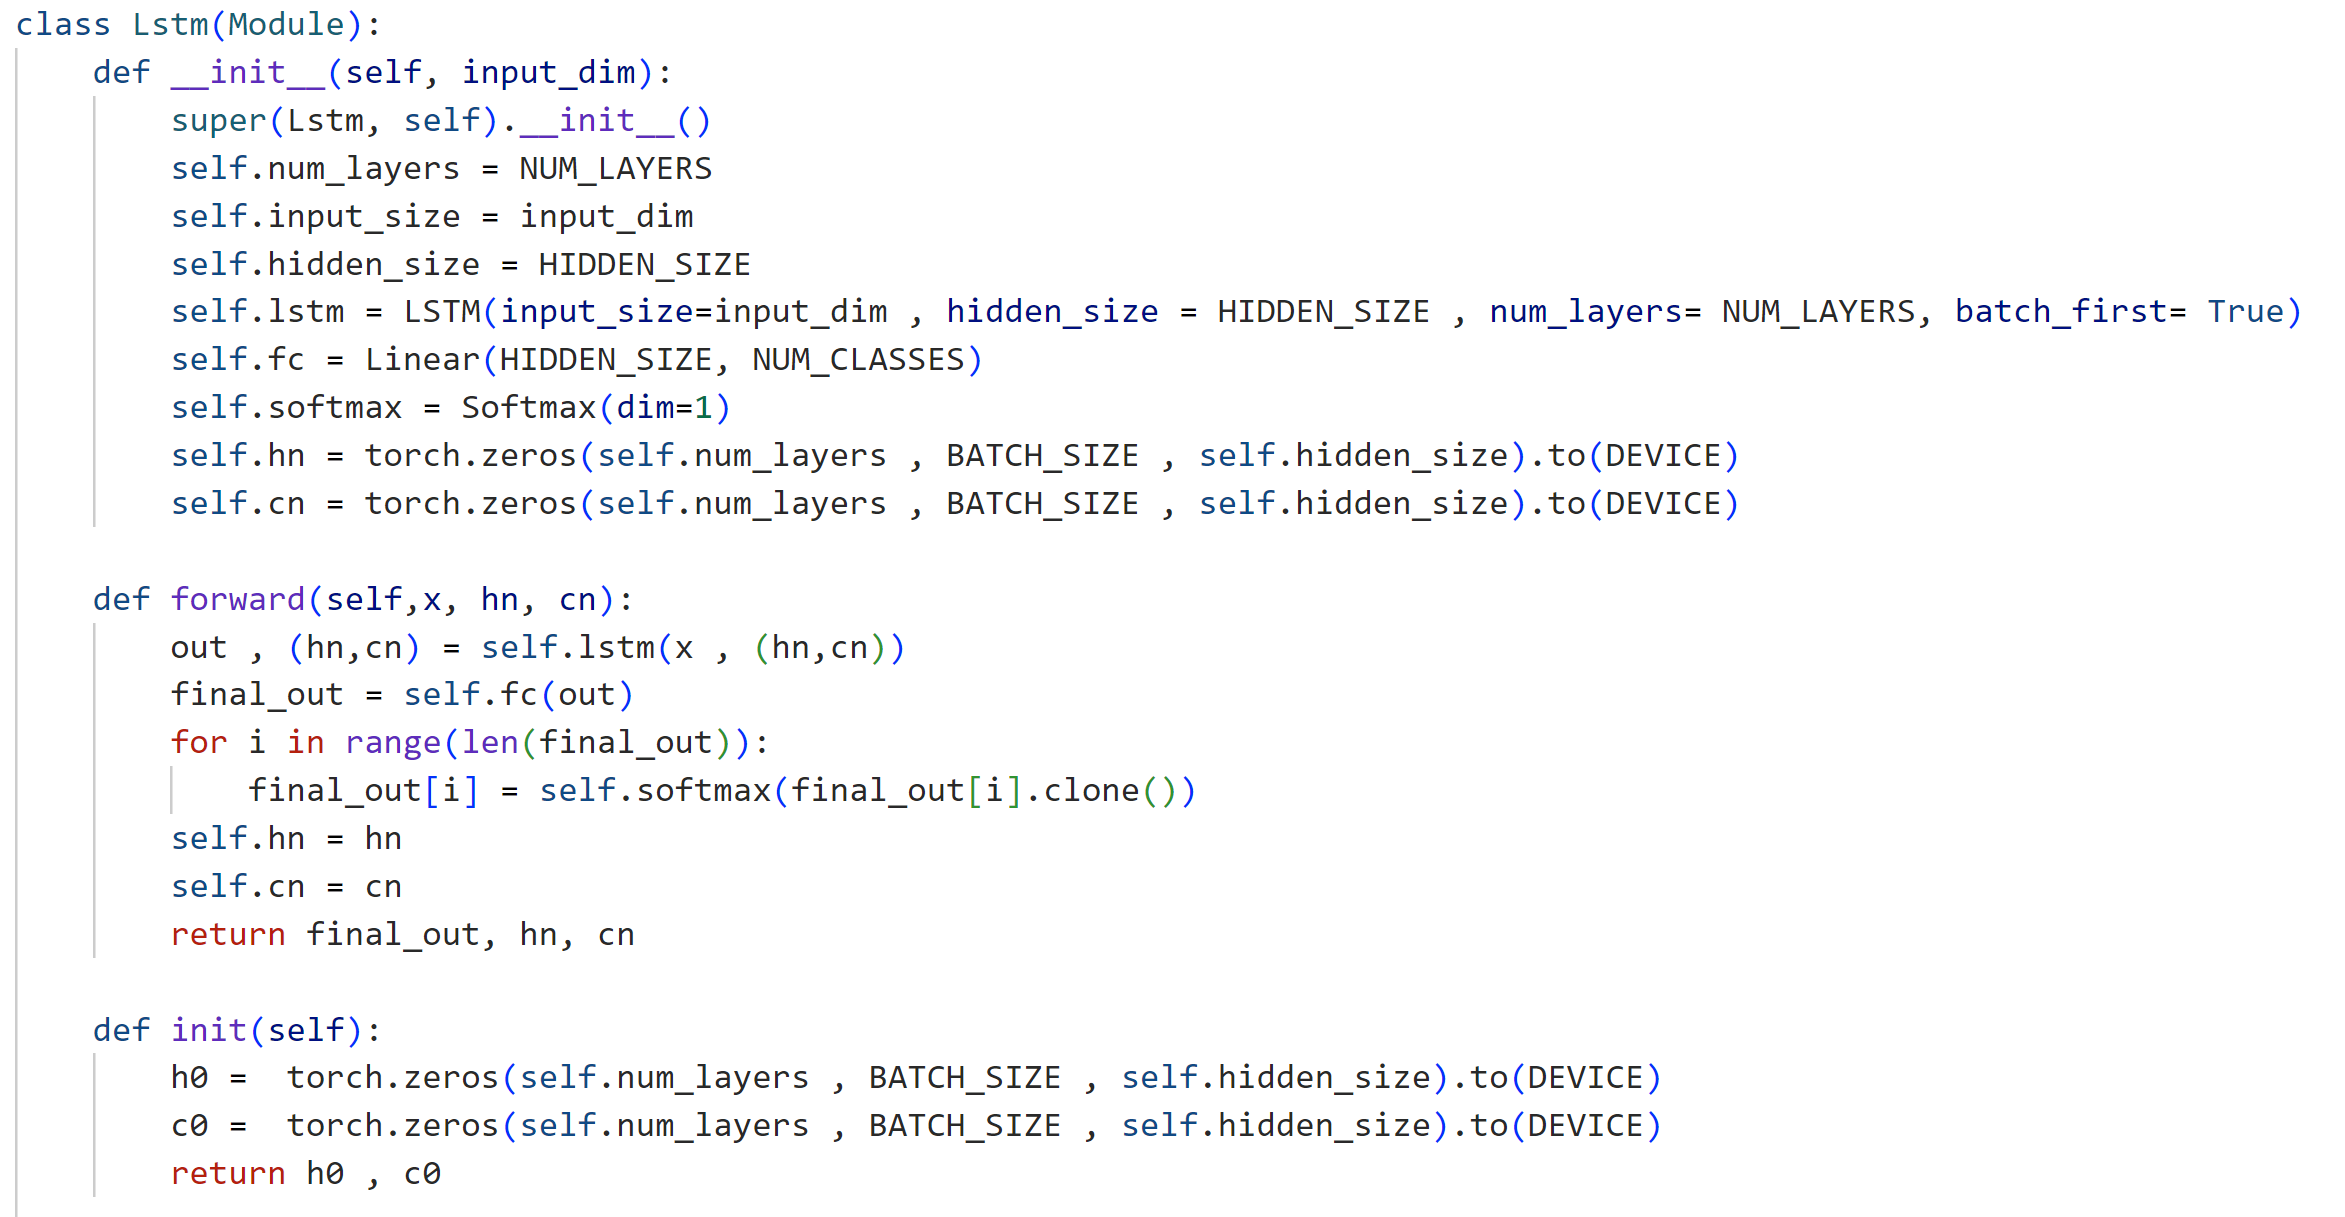
\includegraphics[scale=0.5]{tg1/figuras/codigo.png}
    \caption{Código do modelo LSTM}
    \label{fig:codigo_lstm}
\end{figure}

Os hiperparâmetros são:
\begin{table}[h]
    \centering
    \begin{tabular}{|l|c|l|}
        \hline
        \textbf{Parâmetros} & \textbf{Significado} & \textbf{Valor} \\
        \hline
        NUM\_LAYERS & Número de camadas & 2 \\
        input\_dim & Dimensão da entrada (número de features) &  68\\
        HIDDEN\_SIZE & Tamanho do estado oculto &  60\\
        \hline
    \end{tabular}
    \caption{Parâmetros do Modelo}
    \label{tab:hiperparametros}
\end{table}

Abaixo encontra-se o código do algoritmo de \textit{loss} implementada via Pytorch \cite{Lin_Goyal_Girshick_He_Dollar_2017}.

\begin{figure}[ht]
    \centering
    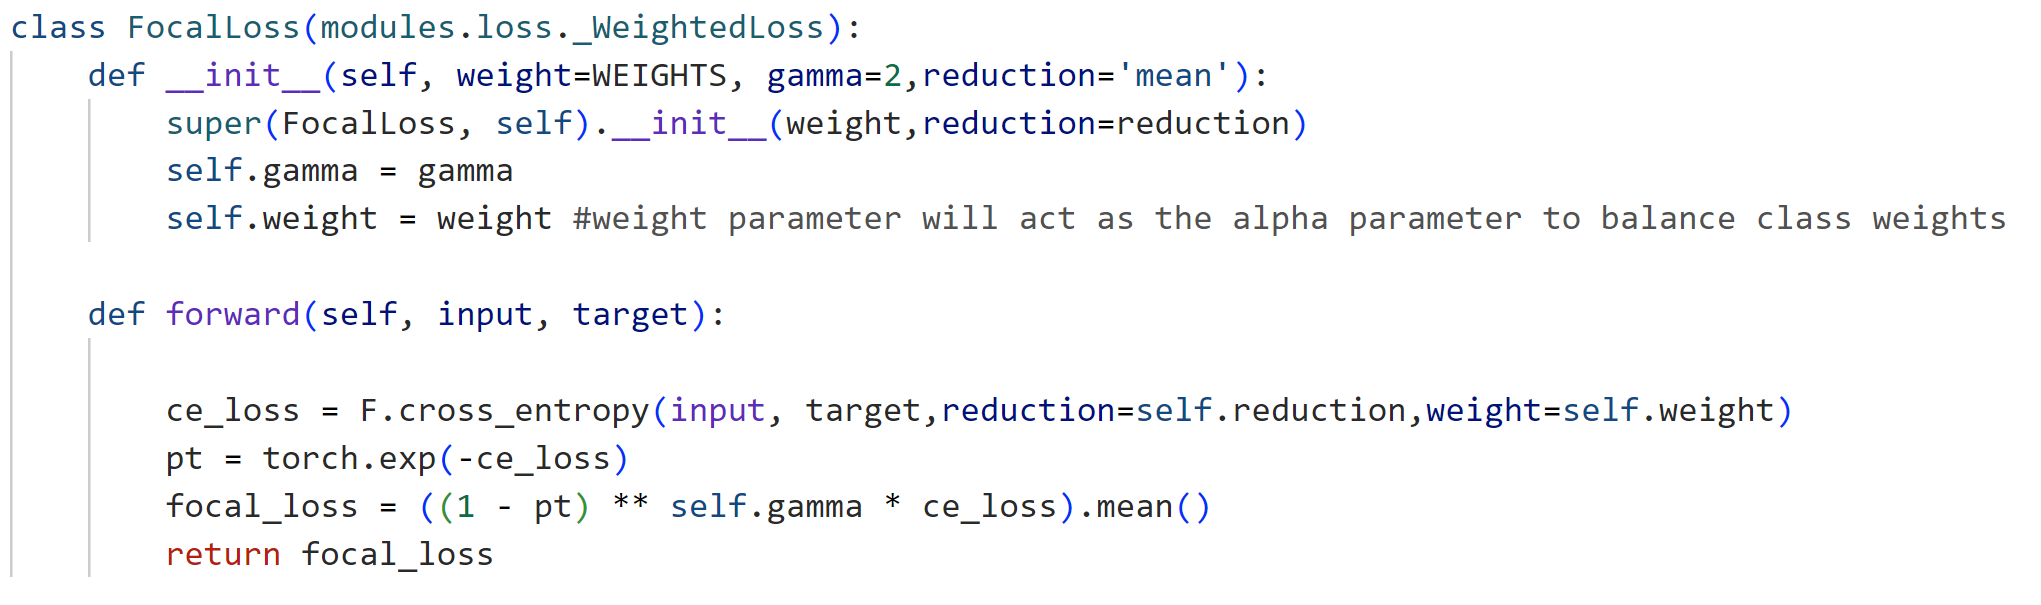
\includegraphics[scale=0.5]{tg1/figuras/loss.png}
    \caption{Código do modelo de Loss Focal}
    \label{fig:loss}
\end{figure}

\subsection{Lidando com Overfitting}
O problema de overfitting foi encontrado durante alguns testes como consequência do mal balanceamento do dataset. A classe 3, referente às queimadas de sub-bosque, representa 1.8\% do dataset, o que resulta em 0\% de acurácia para esta classe para um modelo treinando sem qualquer algoritmo de balanceamento.

É comum na literatura encontrar exemplos de "data augmentation" \cite{survey_data_augmentation}. Trata-se de algoritmos capaz de expandir um dataset sem comprometer de forma significativa seu valor como dado de treinamento. Neste trabalho, optou-se por empregar uma redução de dados como estratégia de balanceamento. Esta estratégia envolve eliminar de forma aleatória dados de rótulos diferentes de forma a se aumentar a representação do tipo de dados de menor presença no dataset. Este tipo de estratégia acabou resultando em overfitting, conforme a imagem a seguir.

\begin{figure}[ht]
    \centering
    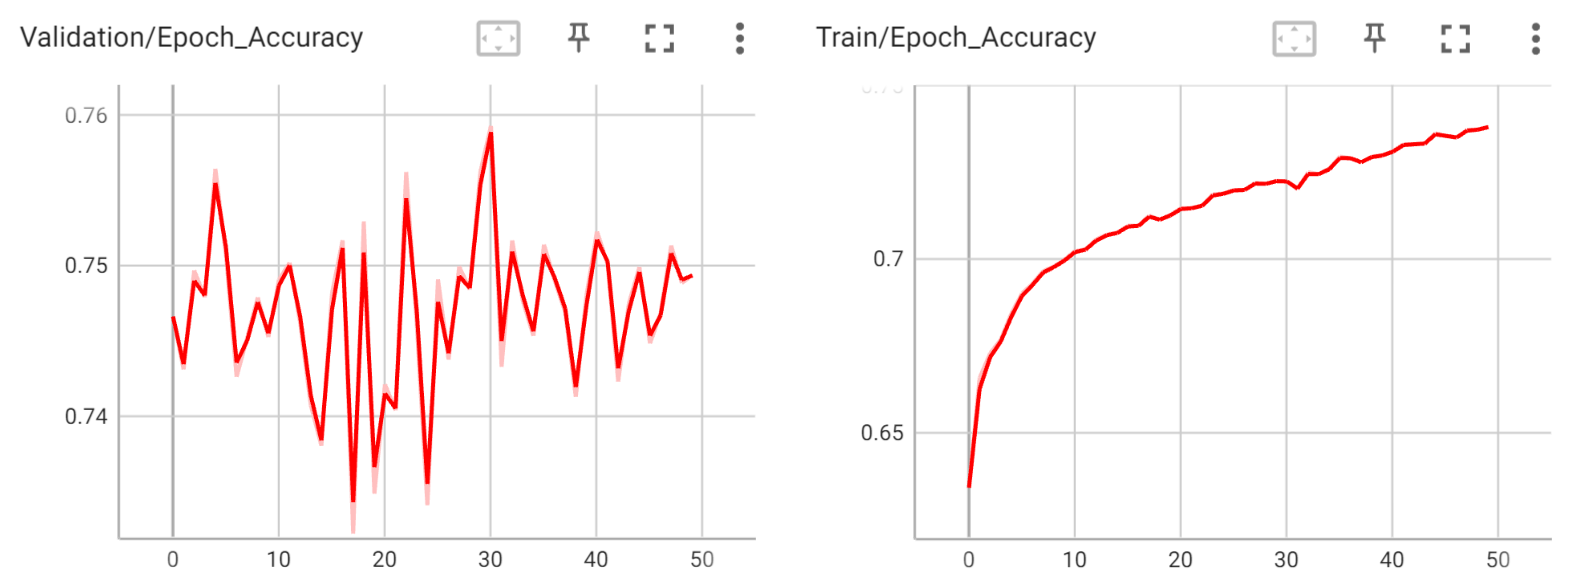
\includegraphics[scale=0.5]{tg1/figuras/overfit.png}
    \caption{Overfitting no treinamento}
    \label{fig:overfitting}
\end{figure}

Na figura \ref{fig:overfitting} pode-se ver que embora a acurácia de treinamento esteja aumentando, a acurácia de validação não está melhorando. Dessa forma, pode-se dizer que a rede está se tornando "viciada" nos dados de treinamento, aprendendo a interpretá-los bem mas não se tornando capaz de prever dados diferentes deste.

Tendo em mãos estes resultados, optou-se por utilizar um leve balanceamento, aumentando a representatividade de 1.8\% para 5\%. Esta proporção foi obtida de forma empírica como um valor que representa uma melhora significativa na acurácia para a classe 3 porém sem reduzir demais a acurácia para as demais classes.


\subsection{Organização em Série Temporal}

Transformar os dados existentes em uma série temporal envolve a adição de uma nova dimensão, a temporal. Em termos práticos, isto é efetuado por meio de uma dimensão acrescentada aos tensores dos dados transformando eventos discretos em dados sequenciais. 

Os dados disponibilizados pelo Censipam possuem identificadores rotulados como "id\_evento". Estes códigos agrupam diferentes detecções de incêndios como pertencentes a um mesmo foco de incêndio e é necessário para a transformação dos dados em uma série temporal. Em outras palavras, cada dados possui três dimensões: o ID representando o foco de incêndio, a quantidade de detecções relativas a este mesmo incêndio, e todos os dados de cada uma destas detecções.

No entanto, esta abordagem envolve o desafio de transformar estes dados em tensores. Todo o código utilizado é construído a partir do Pytorch \cite{NEURIPS2019_9015}, que utiliza tensores como tipo de dado. Tensores são matrizes multi-dimensionais, apenas uma forma de se organizar dados de forma lógica. Por exemplo, pode-se imaginar um tensor tridimensional como um cubo, tratando-se de um tensor cujo as três dimensões são iguais.

Em outras palavras, tensores são uma forma de se estruturar dados de forma regular, onde cada amostra de dados possui dimensões constantes e condizentes com as dimensões do tensor. No entanto, os dados em questão não são regulares pois são obtidos a partir de fenômenos aleatórios e caóticos, de queimadas sobre um território florestal de proporções continentais. Por isso é necessário o emprego de alguma técnica de tratamento de dados que possa regularizá-los, permitindo sua manipulação como tensores.

\subsubsection{Padding}

O desafio em questão é transformar dados de comprimento variado em dados padronizados com o mesmo comprimento, para que possam ser organizados como um tensor tridimensional. Dessarte, é necessário de se empregar um algoritmo capaz de preencher lacunas e eliminar excessos para garantir que todos os dados tenham as mesmas proporções.

"\textit{Padding}" não se trata de um algoritmo específico, mas de qualquer algoritmo capaz de preencher lacunas para garantir regularidade entre dados. Tratando-se de séries temporais, os algoritmos de \textit{Padding} mais comuns envolvem preencher com zeros, com médias ou repetindo valores. Neste trabalho, optou-se por preencher as lacunas repetindo-se a última detecção do evento. 

\begin{figure}[ht]
    \centering
    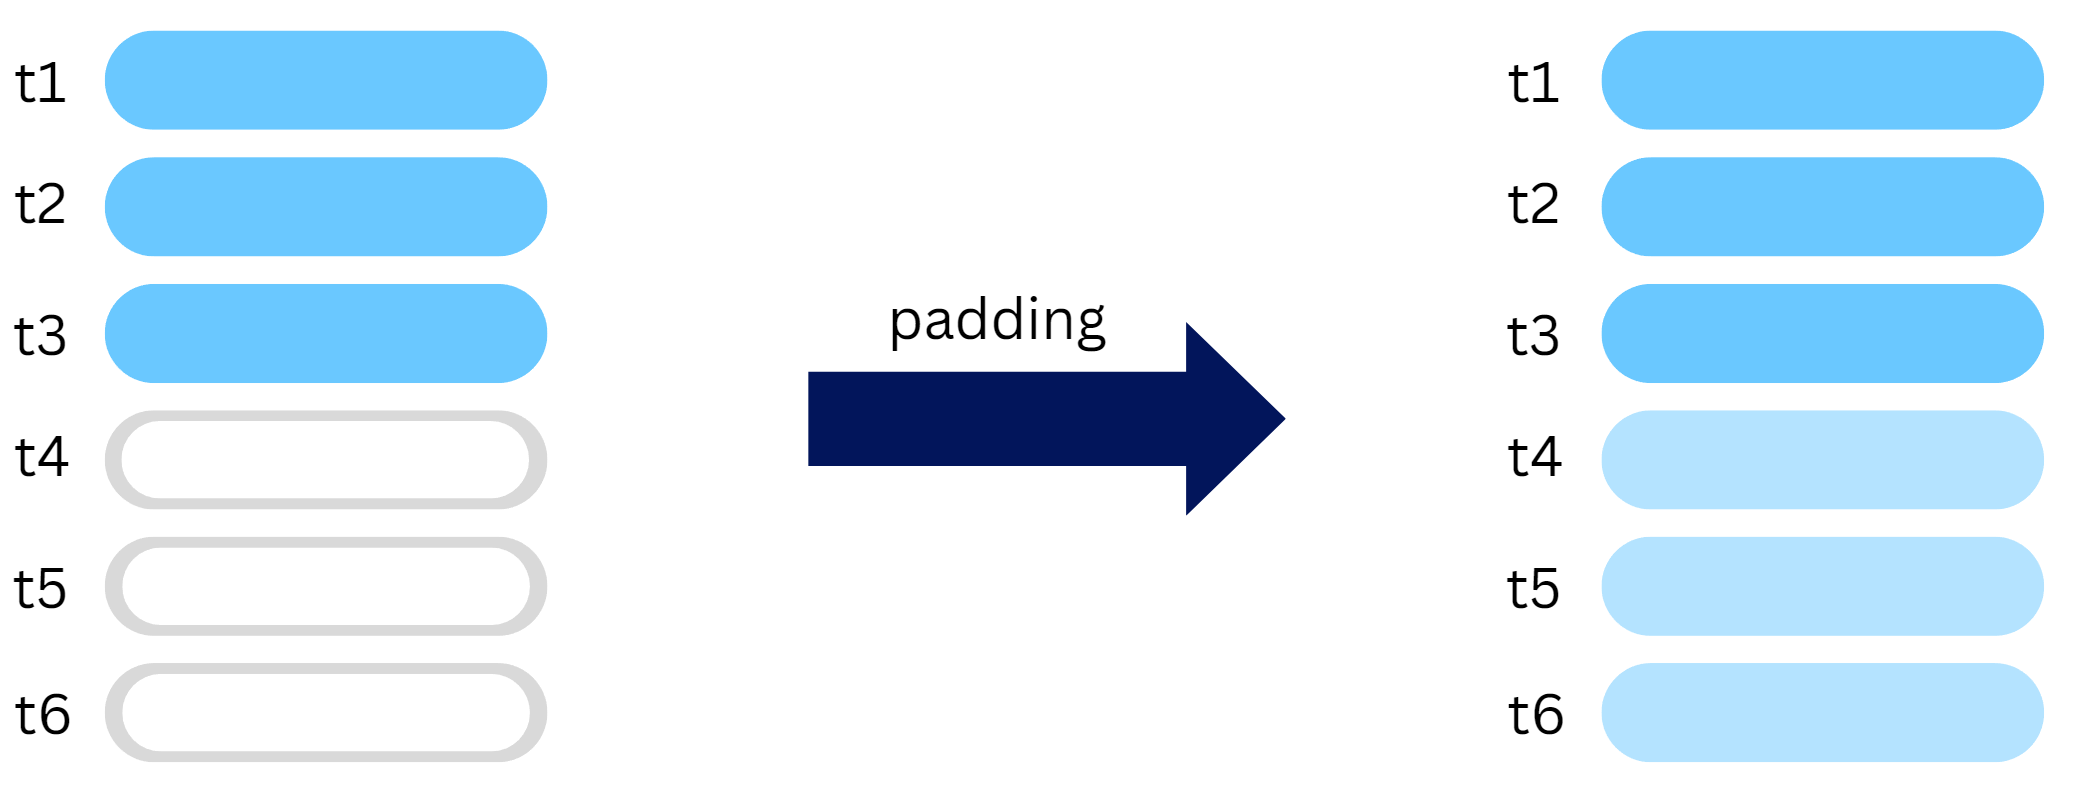
\includegraphics[scale=0.5]{tg1/figuras/padding.png}
    \caption{Representação de Padding}
    \label{fig:padding}
\end{figure}


O motivo para esta escolha é dado pela observação do comportamento da saída da rede ao longo de cada passagem pelos dados. Observou-se que a rede tende ajustar sua saída rapidamente, dentro de 5 iterações, e a manter esta saída até o final, revelando que converge em um valor rapidamente. Logo, foram evitados algoritmos que causem ruído no início da série temporal, período de maior convergência do algoritmo.

\subsection{Metodologia}

Por fim, o funcionamento do código de treinamento pode ser então ilustrado por meio do seguinte fluxograma:
%\todo[inline]{Metodologia toda falando sobre o random forest e nada de lstm, por mim tira esse pedaço e fala sobre LSTM}
%Por meio da biblioteca scikit-learn, é possível escrever um código simples que emprega o uso do modelo Random %Forest e com fácil customização. 

\begin{figure}[H]
	\centering
	\begin{minipage}{0.98\linewidth}
		\centering
		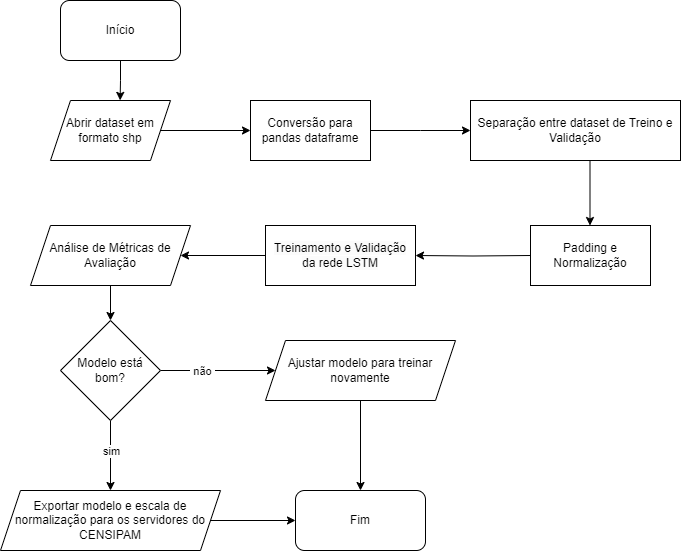
\includegraphics[scale=0.6]{tg1/figuras/flstm_flowchart.png}
		\caption{Fluxograma do funcionamento do código do LSTM} \label{fig:lstm_flowchart}
	\end{minipage}
\end{figure}

\subsection{Desempenho}

No algoritmo de treinamento do modelo, separou-se o dataset entre validação e treinamento, sendo 80\% destinado para o treinamento e 20\% para a validação, separados cronologicamente. As métricas são obtidas de época em época e podem ser observadas por meio do módulo Tensorboard, disponível pelo Tensorflow \cite{tensorflow2015-whitepaper}, ou pelo terminal do programa como uma tabela ao finalizar-se o treinamento, conforme visto na tabela \ref{tab:resultados}.


\todo[inline]{inserir tabela com performance e prints do tensorboard}

    
\begin{table}[h]
    \centering
    \begin{tabular}{|c|c|c|c|c|}
        \hline
        & Acurácia & Precisão & Recall & F1-Score \\
        \hline
        classe 1 & 0.839 & 0.869 & 0.839 & 0.854 \\
        classe 2 & 0.821 & 0.763 & 0.821 & 0.791 \\
        classe 3 & 0 & 0 & 0 & 0 \\
        classe 4 & 0.536 & 0.523 & 0.534 & 0.529 \\
        \hline
        Ponderada & 0.779 & 0.768 & 0.779 & 0.773 \\
        \hline
    \end{tabular}


    \vspace{10pt}
    
    \begin{tabular}{|c|c|}
        \hline
        Classe & Quantidade de eventos \\
        \hline
        classe 1 & 73647 \\
        classe 2 & 64205 \\
        classe 3 & 3136 \\
        classe 4 & 19986 \\
        \hline
    \end{tabular}
    \caption{Resultados da Avaliação}
    \label{tab:resultados}
\end{table}

\subsection{Balanceamento}

Como podemos ver na tabela \ref{tab:resultados}, a rede em seu treinamento praticamente desconsiderou a presença da classe 3 dentro do \textit{dataset}, observando a imagem \ref{fig:lstm_sem_balanc} podemos entender o porque disso. A quantidade de eventos de sub-bosque é bastante inferior a das outras classes, em situações como essa, a rede aprende a não prever aquela classe, isso porque ela é tão inexpressiva que mesmo que ele a desconsidere, a acurácia da rede permanece alta. Como queremos que o trabalho seja capaz de fornecer todas os 4 tipos de fogo, é necessário fazer um balanceamento do \textit{dataset} para aumentar a expressividade das classes menos presentes.

\begin{figure}[H]
	\centering
	\begin{minipage}{0.9\linewidth}
		\centering
		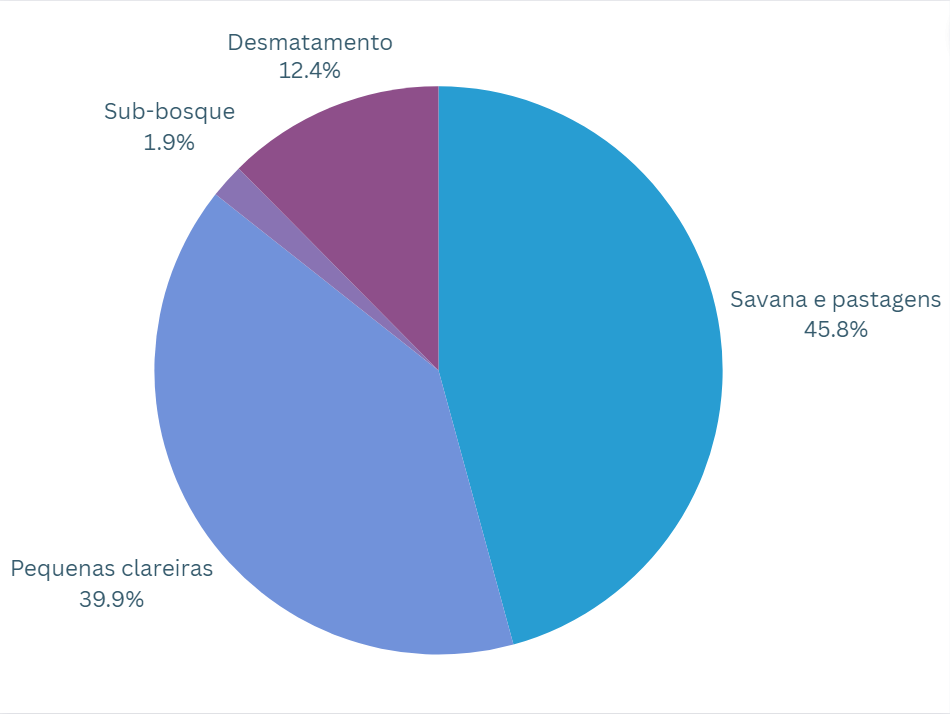
\includegraphics[scale=0.6]{tg1/figuras/sem_balanceamento_pie.png}
		\caption{Gráfico da presença de cada classe dentro do \textit{Dataset}} \label{fig:lstm_sem_balanc}
	\end{minipage}
\end{figure}

O balanceamento pode ser feito utilizando de duas estratégias: remoção de dados e o chamado \textit{data augmentation}, onde aumentamos a quantidade de um certo tipo de dado. Aqui, ambas foram utilizadas, como pode ser observado na tabela \ref{tab:resultados2}, diminuimos a quantidade de eventos para todas as classes exceto a 3, enquanto aumentamos a quantidade de eventos dela. Tal aumento foi feito repetindo os eventos dentro do banco de dados. A tabela também possui o desempenho do modelo para o treinamento com o banco de dados balanceado.

\begin{table}[h]
    \centering
    \begin{tabular}{|c|c|c|c|c|}
        \hline
        & Acurácia & Precisão & Recall & F1-Score \\
        \hline
        classe 1 & 0.795 & 0.904 & 0.795 & 0.846 \\
        classe 2 & 0.804 & 0.772 & 0.804 & 0.788 \\
        classe 3 & 0.290 & 0.237 & 0.289 & 0.261 \\
        classe 4 & 0.620 & 0.485 & 0.619 & 0.544 \\
        \hline
        Ponderada & 0.767 & 0.786 & 0.767 & 0.774 \\
        \hline
    \end{tabular}


    \vspace{10pt}
    
    \begin{tabular}{|c|c|}
        \hline
        Classe & Quantidade de eventos \\
        \hline
        classe 1 & 25088 \\
        classe 2 & 23866 \\
        classe 3 & 9408 \\
        classe 4 & 10662 \\
        \hline
    \end{tabular}
    \caption{Resultados da Avaliação}
    \label{tab:resultados2}
\end{table}

\begin{figure}[H]
	\centering
	\begin{minipage}{0.9\linewidth}
		\centering
		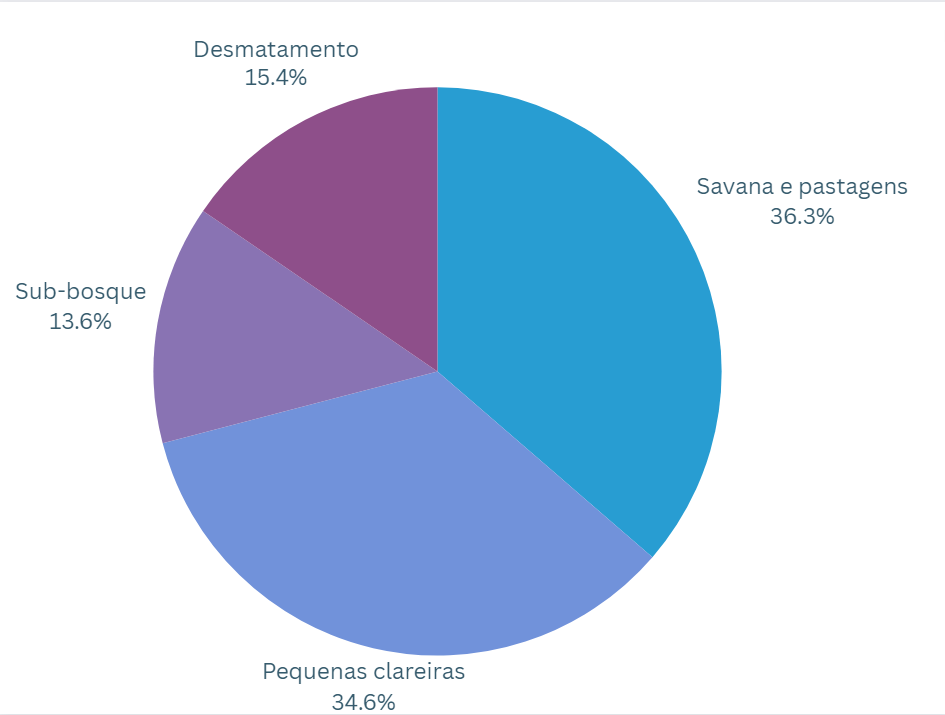
\includegraphics[scale=0.6]{tg1/figuras/balanceado_pie.png}
		\caption{Gráfico balanceado da presença de cada classe dentro do \textit{Dataset}} \label{fig:lstm_com_balanc}
	\end{minipage}
\end{figure}


\section{Servidores do Censipam}

A parceria com o Censipam se deu com o intuito de integrar o modelo de aprendizado como uma ferramenta classificadora em seu sistema. Para isto, foi-se fornecido acesso a uma máquina por meio de tunelamento SSH para que o projeto tenha acesso ao banco de  dados em tempo real.

Dessa forma, o código foi implementado no sistema para que rode continuamente. Atualmente, o programa aguarda até as 23 horas de cada dia para iniciar seu processamento. Neste momento, são requisitados os dados novos, referentes ao dia atual, e os dados antigos de mesmo ID, com apenas XXX features. A partir delas, o algoritmo de adição de features adiciona as demais. Em sequência, os dados passam pela etapa de pré-processamento, sendo normalizados e efetuado o padding. Por fim, o algoritmo de aprendizado de máquina classifica estes dados e monta arquivos dos tipos CSV e SHP com todos os dados classificados.

\subsection{Dados de Treinamento e Dados em Produção}
\todo[inline]{mostrar gráficos comparando ambos datasets}
Os fornecidos para o treinamento do algoritmo e os dados obtidos em produção nos servidores são diferentes. Primeiramente, os dados de treinamento vão até o ano 2022 enquanto os dados disponíveis nos servidores se iniciam em 2023. Além disso, é interessante de se estudar a continuidade entre estes dados, de forma a garantir que sua qualidade é similar à dos dados utilizados no treinamento, ou se houve alguma mudança na forma como são produzidos, como por exemplo, mudança de métrica de metros para quilômetros.


\subsection{Comparando dados do Treinamento com os dados em Produção}

O treinamento do modelo de aprendizado de máquina envolve o uso de um dataset de treino suficientemente parecido com dados de casos práticos, ou aumentam-se as chances de que a performance do modelo em operação não seja satisfatória. Dessa forma, foram-se gerados vários gráficos de caixa comparando as distribuições dos dados utilizados no treinamento com os dados obtidos diretamente dos servidores do Censipam, onde o modelo está em operação diária.

\begin{figure}[H]
	\centering
	\begin{minipage}{0.98\linewidth}
		\centering
		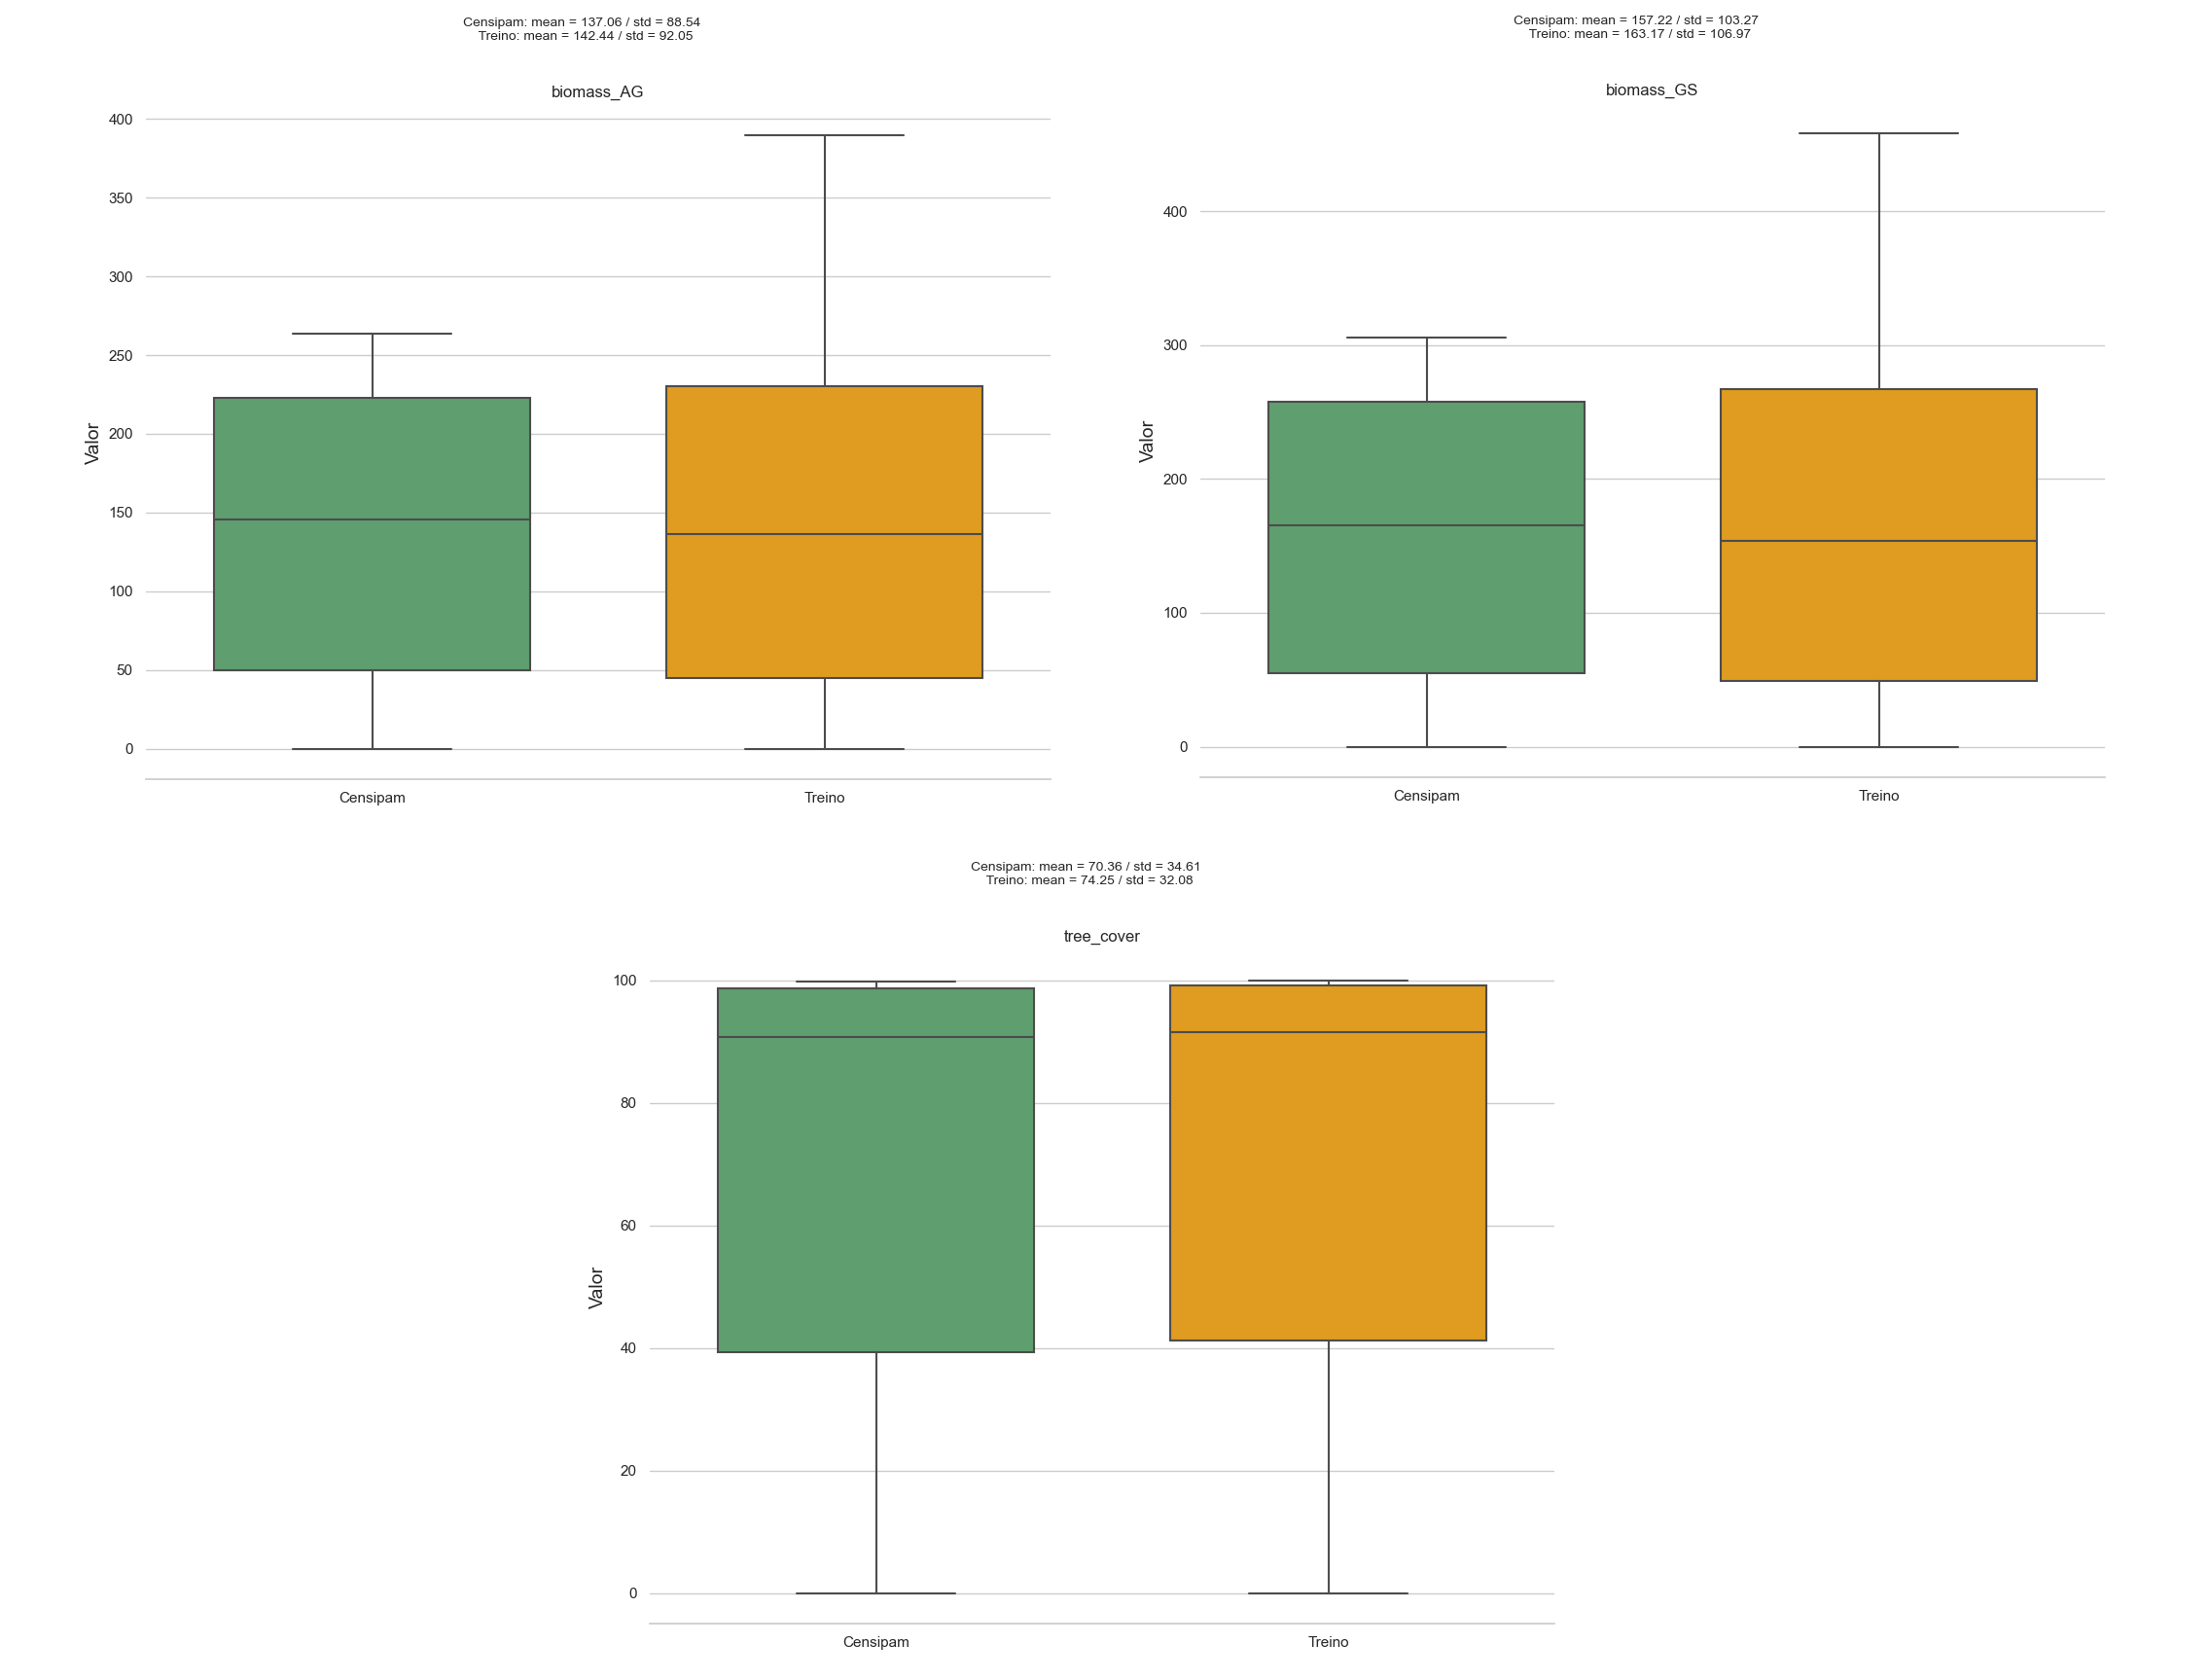
\includegraphics[scale=0.5]{tg1/figuras/graficosbons.png}
		\caption{Diagramas de Caixa de dados semelhantes}
            \label{fig:dadosbons}
	\end{minipage}
\end{figure}

A imagem \ref{fig:dadosbons} contém gráficos de caixa além de média e desvio padrão de algumas \textit{features} cujo as distribuições mostraram-se bastante similares entre os dois datasets. Estes dados possuem distribuições semelhantes, com valores de média e desvio padrão próximos indicando que ambos os dataset se assemelham em relação a estes dados.

No entanto, a diferença entre dados é significativa para vários outros dados. Na imagem \ref{fig:area} encontra-se o gráfico de caixa da \textit{feature} relativa a variação da área do incêndio. A diferença de escala entre as duas medidas é óbvia e indica que há algo de errado nestes dados. Este problema se revela em todos os dados relativos a área.

A escala sugere que talvez os dados estejam em unidades de medida diferentes, uma é metros quadrados e a outra em quilômetros quadrados. A imagem \ref{fig:corrigido} contém o mesmo gráfico, porém com os dados do servidor ajustados de quilômetro quadrado para metro quadrado. Como a semelhança entre os dados é alta, a hipótese de que trata-se de uma diferença de escala utilizada na geração dos dados é provavelmente verdadeira.

\begin{figure}[H]
	\centering
	\begin{minipage}{0.98\linewidth}
		\centering
		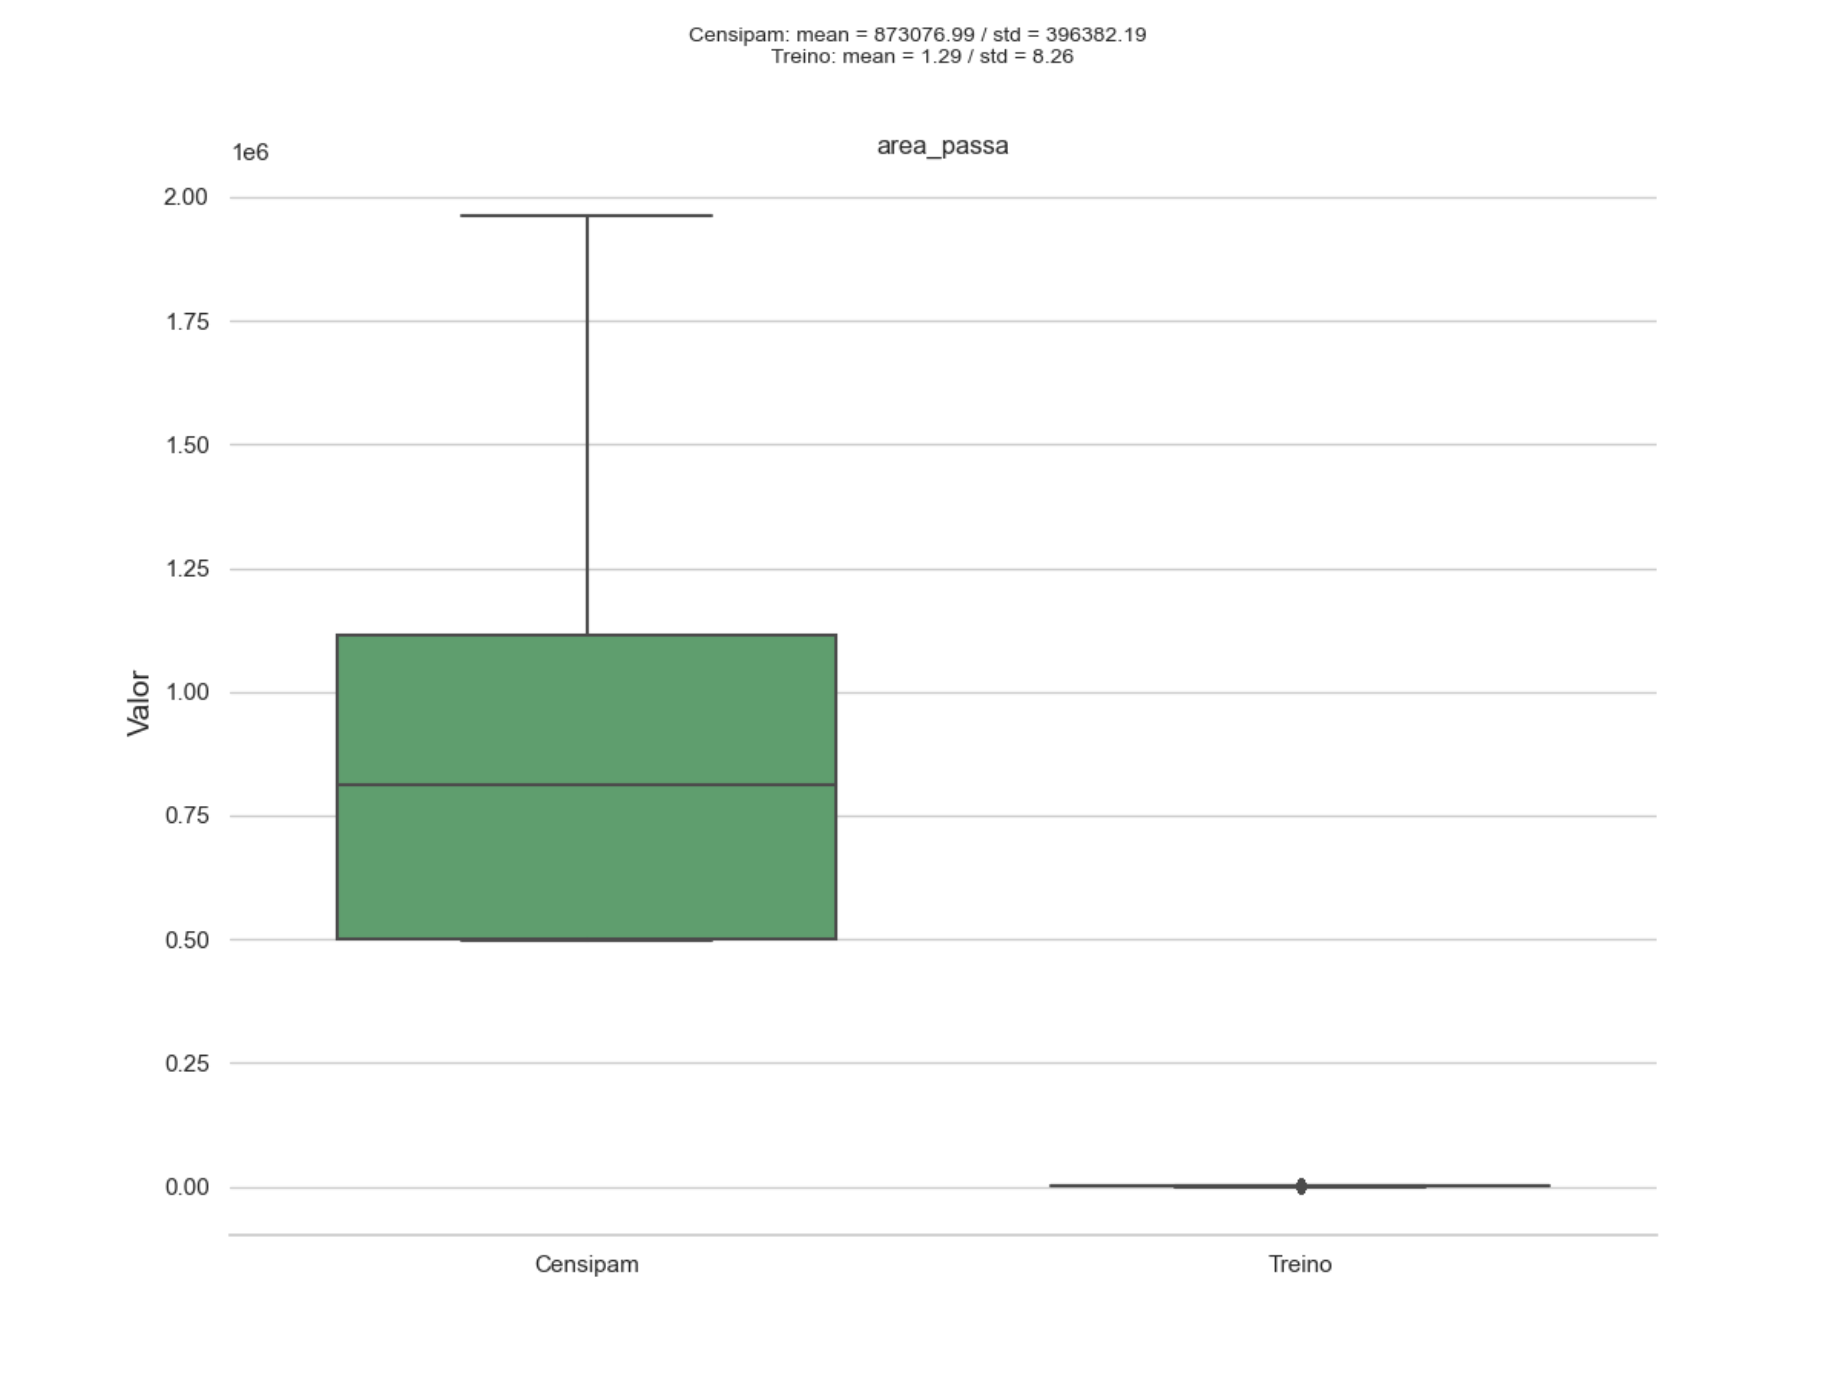
\includegraphics[scale=0.6]{tg1/figuras/area2.png}
		\caption{Diagramas de Caixa de variação de área da queimada}
            \label{fig:area}
	\end{minipage}
\end{figure}


\begin{figure}[H]
	\centering
	\begin{minipage}{0.98\linewidth}
		\centering
		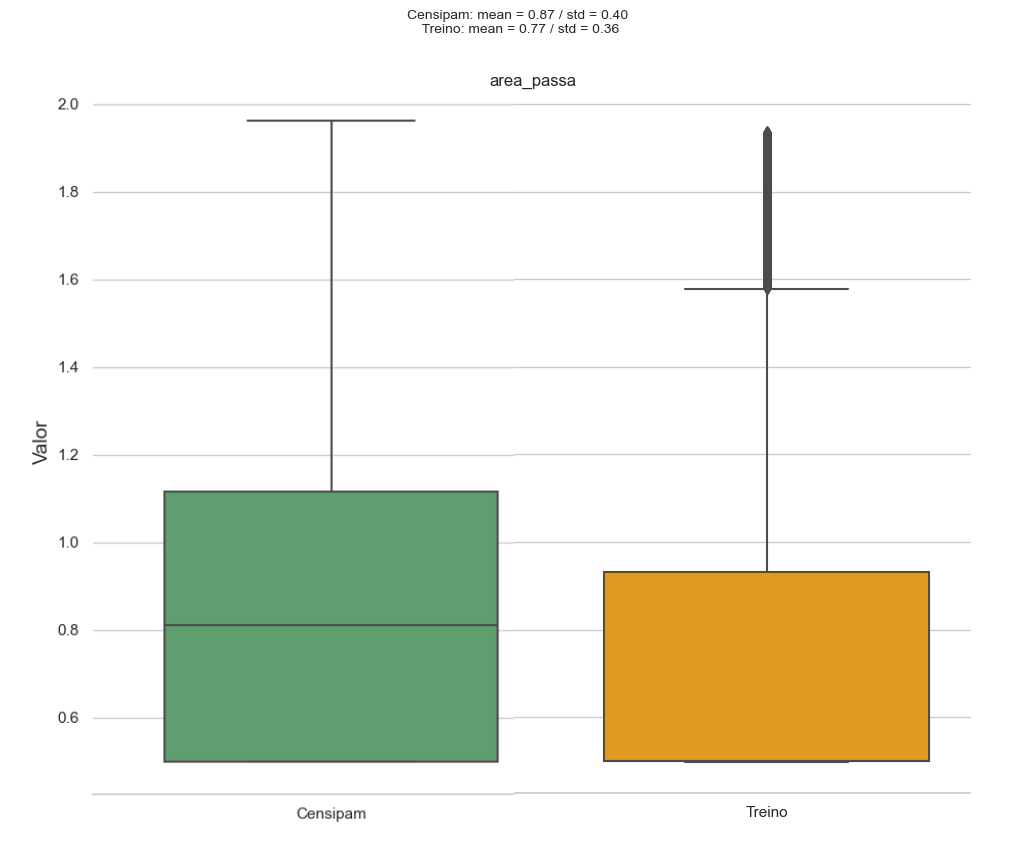
\includegraphics[scale=0.6]{tg1/figuras/corrigido.png}
		\caption{Diagramas de Caixa de variação de área da queimada corrigido em 10e6}
            \label{fig:corrigido}
	\end{minipage}
\end{figure}

Além disto, a \textit{features} geradas costumam apresentar problemas em geral, com todos os dados sendo aproximadamente zero, indicando algum problema com o algoritmo que as gera. Como este erro não surgiu durante o processo de gerar dados para o treinamento, nem ao se gerarem os dados em produção para o trabalho de \cite{BrunoScholess2023}. A hipótese mais provável é de que há alguma diferença nestes dados disponíveis no servidor do Censipam para o projeto atual que não foi levada em consideração durante o desenvolvimento do algoritmo. A inconsistência específica não foi encontrada.

Dessa forma, espera-se que o modelo não performe bem em produção, visto que não está recebendo dados adequados. Até o momento não tem como se verificar sua verdadeira performace visto que os dados novos do servidor não foram rotulados manualmente pelo pessoal do Censipam.





% \section{Evolução do modelo MLP}

% DROP OUT, NORM BATCH, LAYERS, BATCH SIZE, TREINAMENTO, MAQUINA UTILIZADA, ETC

% \section{Análise de Resultados}

% Na última etapa de calculo da precisão do modelo Random Forest, foi obtido os valores da tabela \ref{tab:rf} para quando classificamos o \textit{dataframe} de validação.

% \begin{table}[H]
% \caption{Precisão do modelo Random Forest}
% \label{tab:rf}
% \begin{tabular}{lllll}

%                  & Precision & Recall & F1-score & Quantidade \\
% 0                & 1.00      & 1.00   & 1.00     & 124125  \\
% 1                & 1.00      & 1.00   & 1.00     & 29652   \\
% 2                & 0.84      & 0.73   & 0.78     & 1866    \\
% 3                & 0.86      & 0.92   & 0.89     & 3615    \\
% Acurácia         &           &        & 0.99     & 159258  \\
% Média aritmética & 0.92      & 0.91   & 0.92     & 159258  \\
% Média ponderada  & 0.99      & 0.99   & 0.99     & 159258 
% \end{tabular}
% \end{table}


% A partir do resultado salvo em arquivo .csv, também é possível criarmos uma matriz de confusão para visualizarmos o comportamento da rede, conforme temos na figura \ref{fig:mcrf}. Quantos valores de cada tipo de fogo ela foi capaz de prever corretamente, e quantos ela errou, e para quais valores.

% \begin{figure}[htb]
% 	\centering
% 	\begin{minipage}{0.98\linewidth}
% 		\centering
% 		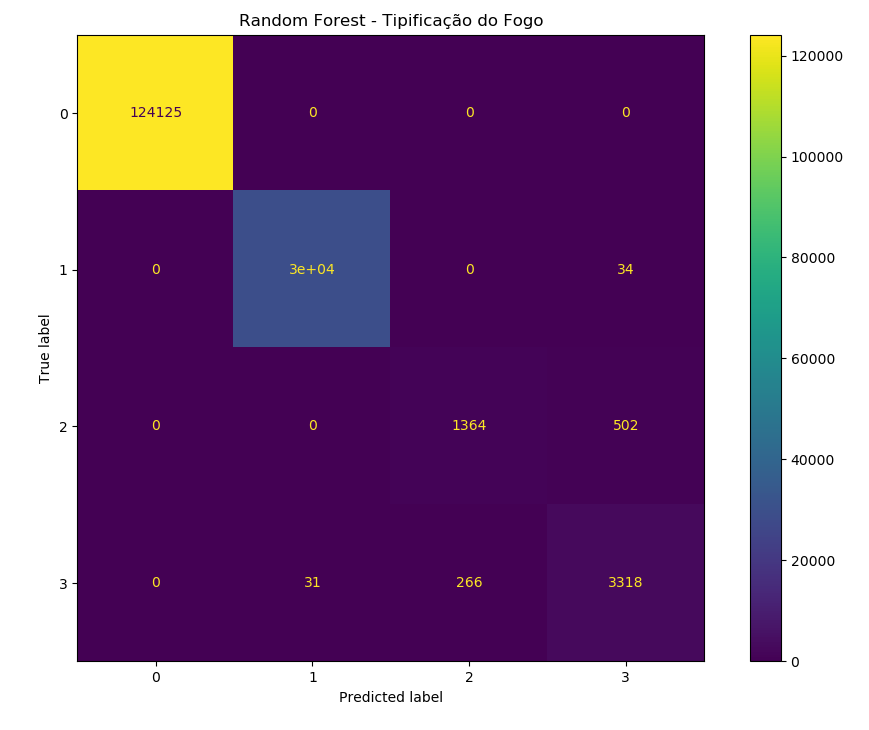
\includegraphics[width=\linewidth]{tg1/figuras/matrizconfusaorandomforest.png}
% 		\caption{Matriz de confusão para Random Forest} \label{fig:mcrf}
% 	\end{minipage}
% \end{figure}

% %\todo{COLOCAR METRICAS DO MLP}

% \begin{table}[H]
% \caption{Precisão do modelo MLP}
% \label{tab:rf}
% \begin{tabular}{lllll}

%                  & Precision & Recall & F1-score & Quantidade \\
% 0                & 1.00      & 1.00   & 1.00     & 124125  \\
% 1                & 0.98      & 1.00   & 0.99     & 29652   \\
% 2                & 0.69      & 0.66   & 0.68     & 1866    \\
% 3                & 0.79      & 0.84   & 0.81     & 3615    \\
% Acurácia         &           &        & ??     & 159258  \\
% Média aritmética & ??      & ??   & ??     & 159258  \\
% Média ponderada  & 0.99      & 0.99   & 0.99     & 159258 
% \end{tabular}
% \end{table}

